\documentclass{beamer}

\usetheme{Copenhagen}

\usepackage{dblfloatfix}
\usepackage{graphicx}
\usepackage{listings}
\usepackage{subfig}
\usepackage{tikz}
\usepackage{xcolor}

\graphicspath{{./assets}}

\begin{document}

\begin{frame}[fragile]
\frametitle{Jared Dyreson}
\begin{itemize}
		\item Cal State Fullerton graduate | December 2021
		\item Contributor to the Tuffix project at CSUF from 2018 to 2021
		\item The way academia meets industry intrigues me
		\item The culture at K \& C aligns with my desires to tinker with new technologies
\end{itemize}

%\begin{frame}{Center positioning}
% create TikZ picture environment
\begin{tikzpicture}[remember picture, overlay]
\node[left=2cm, right=0.75cm, below=1.5cm] at (current page.east) 
{
		
\includegraphics[width=2.5cm]{tuffy}
};
\end{tikzpicture}

\begin{tikzpicture}[remember picture, overlay]
\node[left=3.25cm, below=1.9cm] at (current page.east) 
{
		
\includegraphics[width=2cm]{tux}
};
\end{tikzpicture}
%
\includegraphics[width=2cm]{tux}

%\begin{figure*}[b]%
		%\subfloat{{}}%
		%\qquad
		%\subfloat{{}}%
		%\label{fig:example}%
%\end{figure*}

%\tikz[remember picture, overlay] {\node[anchor=south east, outer sep=0pt] at (current page.south east) {
\includegraphics[width=2.5cm]{tuffy}};}
%\tikz[remember picture, overlay] {\node[anchor=north, outer sep=0pt] at (current page.south east) {
\includegraphics[width=1cm]{tux}};}

\end{frame}

\begin{frame}
\frametitle{Project | Sorting Olympics} 

\begin{itemize}
		\item Sorting algorithm visualizer
		\item Displays one row per `pass' progress of four different sorting algorithms
				\begin{itemize}
						\item Insertion
						\item Merge
						\item Pore's Gold
						\item Quick
				\end{itemize}
		\item Screen is partitioned to have four quadrants for each of the algorithms
		%\item \href{https://www.jareddyreson.xyz/static/demos/Sorting-Olympics/runtime/driver.html?}{\textcolor{blue}{\underline{Demo Link}}}
\end{itemize}

\tikz[remember picture, overlay] {\node[anchor=south east, outer sep=18pt] at (current page.south east) {\href{https://www.jareddyreson.xyz/static/demos/Sorting-Olympics/runtime/driver.html?}{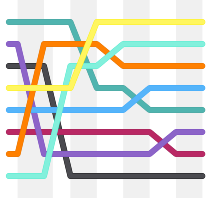
\includegraphics[width=2cm]{sorting}}}}

\end{frame}

\begin{frame}
\frametitle{Input}
\begin{itemize}
		\item Four instances of the same 15-character hexadecimal string in each quadrant
		\item Example:
		
		\begin{figure}[!htpb]
		\centering
		\begin{table}[]
		\begin{tabular}{|l|l|l|l|l|l|l|l|l|l|l|l|l|l|l|}
		\hline
		0 & 5 & C & A & 6 & 2 & 7 & B & C & 2 & B & 6 & F & 0 & 3 \\ \hline
		\end{tabular}
		\end{table}
		\end{figure}
		\item This string is never presorted
		\item Duplicate characters are allowed, `B' for example

\end{itemize}
\end{frame}

\begin{frame}
\frametitle{Output}
\begin{itemize}

		\item Four instances of the same 15-character hexadecimal string each quadrant at each stage of it's sorting phase
		\item These are the states of the strings after one pass
		\item Insertion:
		\begin{figure}[!htpb]
		\begin{table}[]
		\begin{tabular}{|l|l|l|l|l|l|l|l|l|l|l|l|l|l|l|}
		\hline
		0 & 5 & C & A & 6 & 2 & 7 & B & C & 2 & B & 6 & F & 0 & 3 \\ \hline
		\end{tabular}
		\end{table}
		\end{figure}
		
		\item Pore's Gold:
		\begin{figure}[!htpb]
		\begin{table}[]
		\begin{tabular}{|l|l|l|l|l|l|l|l|l|l|l|l|l|l|l|}
		\hline
		0 & 5 & A & C & 2 & 6 & 7 & B & 2 & C & 6 & B & 0 & F & 3 \\ \hline
		\end{tabular}
		\end{table}
		\end{figure}
		
		\item Merge:
		\begin{figure}[!htpb]
		\begin{table}[]
		\begin{tabular}{|l|l|l|l|l|l|l|l|l|l|l|l|l|l|l|}
		\hline
		0 & 5 & A & C & 2 & 6 & 7 & B & 2 & C & 6 & B & 0 & F & 3 \\ \hline
		\end{tabular}
		\end{table}
		\end{figure}
		\item Quick:

		\begin{figure}[!htpb]
		\begin{table}[]
		\begin{tabular}{|l|l|l|l|l|l|l|l|l|l|l|l|l|l|l|}
		\hline
		0 & 2 & 2 & 0 & 3 & 5 & 7 & B & C & C & B & 6 & F & A & 6 \\ \hline
		\end{tabular}
		\end{table}
		\end{figure}
\end{itemize}
\note{Here is a note I want to see}
\end{frame}

\begin{frame}{Success Criteria}

\begin{itemize}
\item All strings are sorted; no strings are never unsorted
\item There can exist a state where some strings are sorted and others are not
		\item The program will continue to loop to new input without user intervention when the success criteria is met
		\end{itemize}

		\end{frame}


\begin{frame}{My Contributions}
\begin{itemize}
		\item Created the visual schema
		\item Designed a small API between P5JS and our project to allow for standardized drawing
		\item Implemented functions to `blit' text to the display
		\item Authored Quick Sort as an iterative solution
		\item As project lead, coordinated meetings and delegated tasks to other team members
\end{itemize}

\begin{tikzpicture}[remember picture, overlay]
\node[left=3cm, right=1.25cm, below=2cm] at (current page.east) 
{
		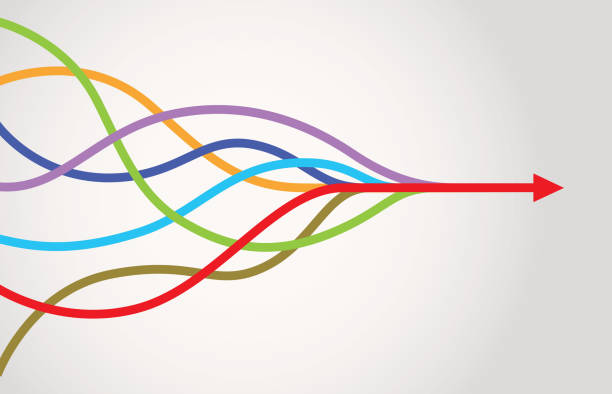
\includegraphics[width=3cm]{contributions}
};
\end{tikzpicture}


\end{frame}

\begin{frame}{Conclusions \& Recommendations}
\begin{itemize}
		\item I was surprised at how much I enjoyed this project and how it influenced other works
		\item It inspired other projects in later classes, such as game design
		\item Could be used as an asset to creating new sorting algorithms
		\item A more functional approach with less abstraction would have been cleaner
		\item Code base likely requires refactoring
		\item Potential for recursive solutions for each sorting algorithm implementation
		\item Compile to WASM to support more algorithms in parallel
\end{itemize}
\end{frame}

\begin{frame}

\begin{center}
\textbf{\Large Questions?}
\end{center}

\end{frame}

\end{document}

